\chapter{Vlastnosti a aplikace nanočástic}

Velikost nanotechnologií je v oblasti velikosti makromolekul (DNA, protilátky) a virů. Nanotechnologie jsou složeny z relativně malého počtu molekul oproti makroskopickým materiálům. Zásadní vlastností a ve většině případů také výhodou je jejich odlišné chování od týchž makroskopických materiálů. Nanomateriály mají specifické fyzikálně-chemické vlastnosti - optické, magnetické, elektrické či mechanické vlastnosti, reaktivitu a toxicitu. Zmenšení částic způsobuje zvětšení povrchu a současně dochází ke zvýšení Gibbsovy volné energie a tedy reaktivitě nanočástic. Reaktivita také koreluje s počtem molekul/atomů na povrchu materiálu. Vlastnosti částic ovlivňuje také povrchový náboj, chemické složení povrchu, tvar povrchu a jeho defekty či porozita. Specifikem nanočástic je také jejich shlukování do aglomerátů (shluky slabě vázaných částic nebo agregátů) či agregátů (shluky pevně vázaných nebo sloučených částic, jejich povrch je přibližným součtem povrchu jednotlivých komponent) a tím jejich zvětšování. \cite{nohavica2011,filipova2012}  \\

Nanomateriály jsou přirozenou součástí životního prostředí. Přirozené nanomateriály vznikají při sopečných erupcích a požárech. Základní klasifikace nanomateriálů rozlišuje
    \begin{itemize}
        \item nanočástice vzniklé jako nežádoucí produkt jiného procesu
        \item nanočástice uměle připravené pro určitou aplikaci
    \end{itemize}
    
Vznik nanočástic doprovází hoření benzinu, plynu nebo nafty ve spalovacích motorech, topení fosilními palivy, hoření v leteckých motorech, spalování odpadu a další. Tyto procesy jsou velkými znečišťovately životního prostředí a podporují vznik nejrůznějších forem rakoviny. \cite{nohavica2011}\\

Uměle připravované nanočástice lze rozdělit do čtyř kategorií dle postupného příchodu na ekonomický trh. Přehlednou časovou osu ukazuje obrázek \ref{fig:casova_osa_nanocastic}. Rozlišujeme pasivní nanostruktury (dispergované nanostruktury a produkty využívající nanostruktury), aktivní nanostruktury (bioaktivní nanostruktury a fyzikálně-chemicky aktivní nanostruktury), systémy nanosystémů (nanorobotika) a molekulární nanosystémy (molekulární nanostroje). \cite{filipova2012}

    \begin{figure}
        \centering
        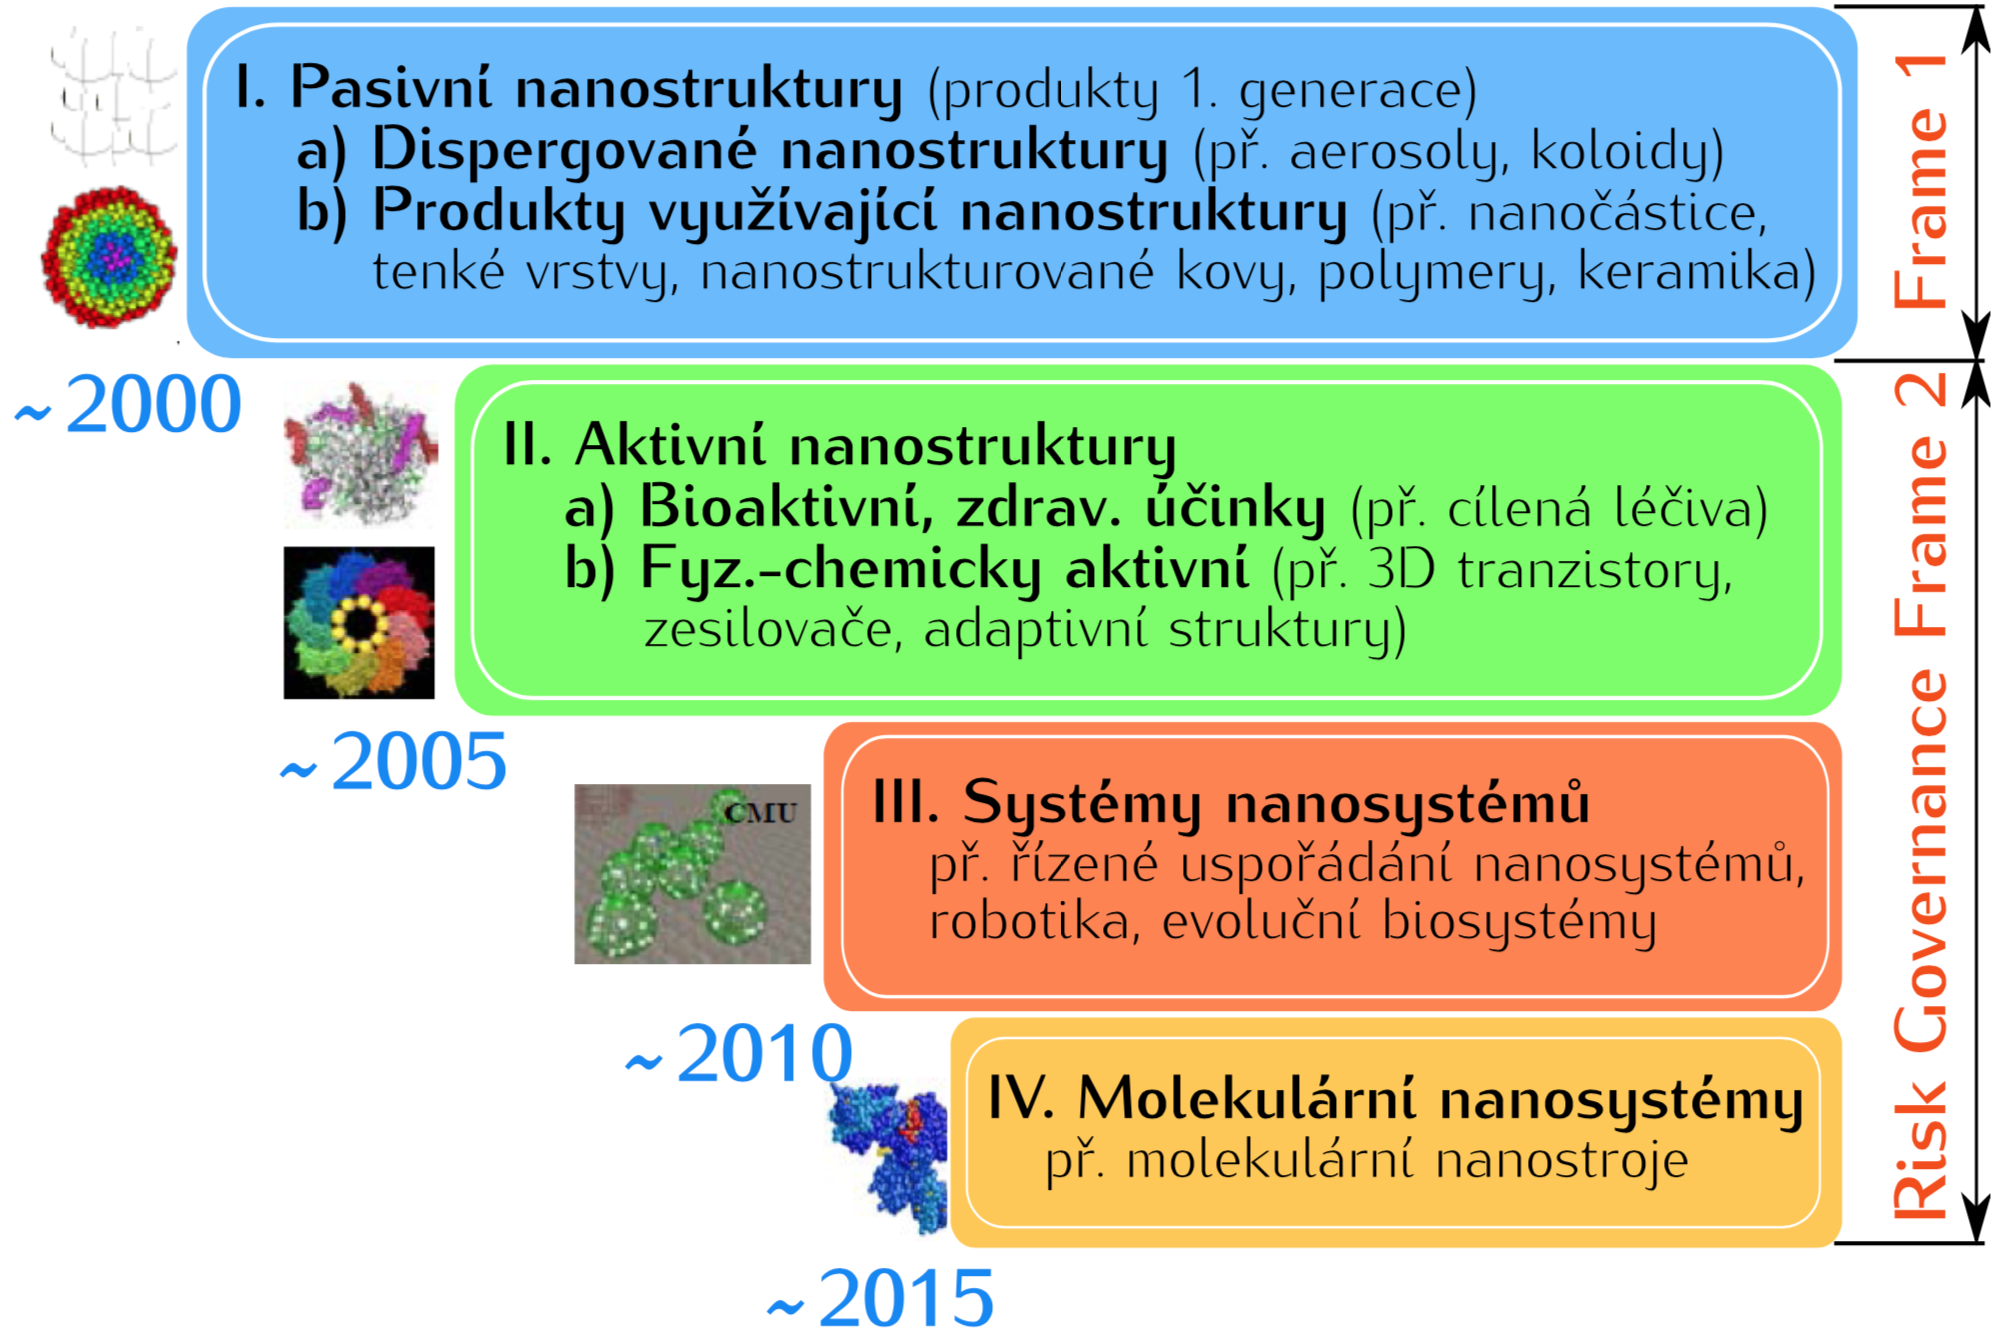
\includegraphics[width=0.9\textwidth]{pictures/casova_osa_generaci_nanomaterialu.png}
        \caption{Časový přehled průmyslového využití nanotechnologií. \cite{filipova2012}}
        \label{fig:casova_osa_nanocastic}
    \end{figure}

\section{Medicínské aplikace}

    V oblasti medicíny se využívají nanočástice k cílenému přenosu léčiv v lidském organismu. Především léčba rakoviny se ubírá směrem přesného cílení chemoterapeutik do tumorové tkáně. Velkou výhodou je snížení vedlejších účinků a nižší zasažení zdravé tkáně. \cite{nanoprotech2016} Nanonosiče také umožňují řízené a postupné uvolňování léčiva po dlouho dobu. Díky malé velikosti léčiva také mohou prostupovat hematoencefalickou bariérou a mohou se tak dostat až k nervovým zakončením v mozku. Důležitou aplikací je také dezinfekce - mnoho nanomateriálů působí antibakteriálně. \cite{nohavica2011}


\section{Strojírenské, stavebnické a auto-moto aplikace}

    Díky nanomateriálům lze vyrobit konstrukční materiály s výbornými vlastnostmi. Materiály, které jsou pevnější a odolnější a současně lehčí či pružnější. Jednu z nejdelších tradic mají různé nanonátěry, které působí antikorozně či izolačně, snižují tření, ochraňují lak či působí antibakteriálně. Mohou původním materiálům propůjčovat voděodolnost nebo je chránit před UV zářením. \cite{nanoprotech2016,nasiol}

\section{Elektronika}

    Zlepšení fyzikálních vlastností nanomateriálů umožňuje zmenšení záznamových zařízení a počítačů. Promítá se do konstrukce palivových článků, fotovoltaických článků, monitorů a televizí. Pracuje se na využití supravodivých materiálů za pokojové teploty. Konstruují se různé biosenzory a elektronické součástky \cite{filipova2012,nanoprotech2016} 

\section{Chemický průmysl}

    Aplikace nanomateriálů v chemickém průmyslu se zaměřují především na účinnější a efektivnější čištění vod, průmyslových roztoků a další dekontaminační technologie. Vysokého povrchu nanočástic se využívá ke katalytickým účinkům, sorpčním aplikacím a chemickým senzorům. \cite{nanoprotech2016,understanding_nano} 

\section{Vojenský průmysl}

    Vojenský průmysl využívá vysoké odolnosti nanomateriálů a jejich nízké hmotnosti. Z uhlíkových nanovláken se vyrábí lehké neprůstřelné materiály či konstrukce ultralehkých letadel. Dále se využívají speciální senzory a elektronika.  \cite{nanoprotech2016}
    
\section{Budoucnost nanomatechnologií}

   V roce 2010 se předpokládalo, že od roku 2020 budou produkty nanotechnologií využívány téměř ve všech průmyslových sektorech a oblastech medicíny, v informačních technologiích a ochraně přírody. \cite{filipova2012} Tento trend můžeme již v roce 2019 potvrdit. Také státní inovační strategie podporují další rozvoj nanotechnologií. 